\documentclass[a4paper, 14pt]{extarticle}

%--------------------------------------
%               Пакеты
%--------------------------------------
\usepackage{geometry}
\geometry{a4paper,tmargin=2cm,bmargin=2cm,lmargin=3cm,rmargin=1cm}

\usepackage[T2A]{fontenc}
\usepackage[utf8]{inputenc}
\usepackage[english, main=russian]{babel}

\usepackage{textcomp}
\usepackage{indentfirst}
\usepackage{graphicx}
\graphicspath{{./images/}}
\usepackage{wrapfig}
\usepackage{enumitem}
\usepackage{caption}
\usepackage{hyperref}
\hypersetup{unicode=true}

\DeclareCaptionLabelSeparator*{emdash}{~--- }
\captionsetup[figure]{labelsep=emdash,font=onehalfspacing,position=bottom}

\usepackage{tempora}
\usepackage{amsmath}
\usepackage{color}
\usepackage{listings}

\lstset{
  belowcaptionskip=1\baselineskip,
  breaklines=true,
  frame=L,
  xleftmargin=\parindent,
  language=C++,
  showstringspaces=false,
  basicstyle=\footnotesize\ttfamily,
  keywordstyle=\bfseries\color{blue},
  commentstyle=\itshape\color{purple},
  identifierstyle=\color{black},
  stringstyle=\color{red},
  numbers=left,
  numberstyle=\tiny,
  stepnumber=1,
  numbersep=5pt
}

\linespread{1.3}
\sloppy
\clubpenalty=10000
\widowpenalty=10000

%--------------------------------------
%               Документ
%--------------------------------------
\begin{document}

%--------------------------------------
%           Титульный лист
%--------------------------------------
\begin{titlepage}
\thispagestyle{empty}

\vspace*{-60pt}
\hspace{-65pt}
\begin{minipage}{0.3\textwidth}
  \hspace*{-20pt}\centering
  
\includegraphics[width=\textwidth]{emblem}
\end{minipage}
\begin{minipage}{0.67\textwidth}\small\bfseries
  \vspace*{-0.7ex}
  \centerline{Министерство науки и высшего образования Российской Федерации}
  \vspace*{-0.7ex}
  \centerline{Федеральное государственное бюджетное образовательное учреждение}
  \vspace*{-0.7ex}
  \centerline{высшего образования}
  \vspace*{-0.7ex}
  \centerline{<<Московский государственный технический университет}
  \vspace*{-0.7ex}
  \centerline{имени Н.\,Э.~Баумана}
  \vspace*{-0.7ex}
  \centerline{(национальный исследовательский университет)>>}
  \vspace*{-0.7ex}
  \centerline{(МГТУ им.\,Н.\,Э.~Баумана)}
\end{minipage}

\vspace{-25pt}
\hspace{-35pt}\rule{\textwidth}{2.3pt}
\vspace*{-20.3pt}
\hspace{-35pt}\rule{\textwidth}{0.4pt}

\vspace{1.5ex}
\hspace{-35pt}\small
\noindent ФАКУЛЬТЕТ\hspace{80pt} <<Информатика и системы управления>>
\vspace*{-16pt}
\hspace{47pt}\rule{0.83\textwidth}{0.4pt}

\vspace{0.5ex}
\hspace{-35pt}\small
\noindent КАФЕДРА\hspace{50pt} <<Прикладная математика и информатика>>
\vspace*{-16pt}
\hspace{30pt}\rule{0.866\textwidth}{0.4pt}

\vspace{11em}
\begin{center}
  \Large\bfseries Лабораторная работа № 8\\[1ex]
  \large по курсу <<Языки и методы программирования>>\\[1ex]
  \large <<Разработка шаблона класса>>
\end{center}

\vspace{8em}
\begin{flushright}
  Студент группы ИУ9-21Б \textbf{Хромов М.\,А.}\\[2ex]
  Преподаватель \textbf{Посевин Д.\,П.}
\end{flushright}

\vfill
\begin{center}
  \textsl{Москва 2025}
\end{center}
\end{titlepage}

%--------------------------------------
\section{Задание}\label{sect:task}
Согласно выбранному из таблиц 1–16 описанию требуется составить \textbf{шаблон класса}, разместив его в отдельном заголовочном файле. Проверку работоспособности класса необходимо организовать в функции \lstinline|main|, помещённой в файле \texttt{main.cpp}.

%--------------------------------------
\section{Индивидуальный вариант}\label{sect:variant}
\begin{description}[leftmargin=0pt]
  \item[Equality\textless T, N\textgreater] линейное равенство 
        \[
          a_1x_1 + a_2x_2 + \dots + a_Nx_N = b,
        \]
        где коэффициенты $a_i$ и $b$ имеют тип~\lstinline|T|.\
        Требуется операция проверки, удовлетворяет ли заданный вектор значений переменных равенству.\
        При $N=1$ добавить операцию решения уравнения.
  \item[IntPQueue\textless L, H\textgreater] приоритетная очередь для целых чисел диапазона $[L,\,H]$ с обычным набором операций.\
        Если $H-L+1 \le 256$, структура должна храниться во \emph{массиве} \lstinline|char|.
\end{description}

%--------------------------------------
\section{Практическая реализация}\label{sect:impl}
Ниже приведены исходные тексты пяти шаблонных классов с примерами использования.
Для файлов, превышающих 80 строк кода, реализация разбита на две части.

\subsection*{Листинг 1. \texttt{main.cpp} (тест двусвязного списка)}
\begin{figure}[!htb]
\begin{lstlisting}[language=C++,caption={main.cpp для \texttt{List<int>}},label={lst:list1}]
#include <iostream>
#include "list_int.h"
using namespace std;

int main() {
    List<int> myList;

    cout << "Добавляем элементы:" << endl;
    myList.insert(5, 0);
    myList.insert(10, 1);
    myList.insert(15, 1);          // вставка на позицию 1
    myList.print();

    cout << "Поиск элементов:" << endl;
    cout << (myList.find(10)  ? "Найдено" : "Не найдено") << endl;
    cout << (myList.find(100) ? "Найдено" : "Не найдено") << endl;

    cout << "Удаление элемента 10:" << endl;
    myList.remove(10);
    myList.print();

    cout << "Сумма элементов:" << endl;
    cout << myList.sum() << endl;
    return 0;
}
\end{lstlisting}
\end{figure}
\clearpage
\subsection*{Листинг 2. \texttt{list\_int.cpp} --- часть 1/2}
\begin{figure}[!htb]
\begin{lstlisting}[language=C++,caption={\texttt{List<int>} — реализация, строки 1–80},label={lst:list2a},firstnumber=1,lastline=80]
#include "list.h"

template <>
class List<int> {
private:
    struct Node {
        int data;
        Node* next;
        Node* prev;
    };

    Node* head;
    Node* tail;

public:
    List();
    ~List();

    void insert(int value, int position);
    bool find(int value);
    void remove(int value);
    void print();
    int sum();
};

List<int>::List() {
    head = nullptr;
    tail = nullptr;
}

List<int>::~List() {
    Node* current = head;
    while (current != nullptr) {
        Node* temp = current;
        current = current->next;
        delete temp;
    }
}

void List<int>::insert(int value, int position) {
    Node* newNode = new Node{value, nullptr, nullptr};

    if (head == nullptr) {
        head = tail = newNode;
        return;
    }

    if (position <= 0) {
        newNode->next = head;
        head->prev = newNode;
        head = newNode;
        return;
    }

    Node* current = head;
    int index = 0;
    while (current->next != nullptr && index < position - 1) {
        current = current->next;
        index++;
    }

    if (current->next == nullptr) {
        current->next = newNode;
        newNode->prev = current;
        tail = newNode;
    } else {
        newNode->next = current->next;
        newNode->prev = current;
        current->next->prev = newNode;
        current->next = newNode;
    }
}
\end{lstlisting}
\end{figure}
\clearpage
\subsection*{Листинг 3. \texttt{list\_int.cpp} --- часть 2/2}
\begin{figure}[!htb]
\begin{lstlisting}[language=C++,caption={\texttt{List<int>} — реализация, строки 81–129},label={lst:list2b},firstnumber=81]
bool List<int>::find(int value) {
    Node* current = head;
    while (current != nullptr) {
        if (current->data == value) {
            return true;
        }
        current = current->next;
    }
    return false;
}

void List<int>::remove(int value) {
    Node* current = head;
    while (current != nullptr) {
        if (current->data == value) {
            if (current == head) {
                head = current->next;
                if (head != nullptr) {
                    head->prev = nullptr;
                } else {
                    tail = nullptr;
                }
            } else if (current == tail) {
                tail = current->prev;
                tail->next = nullptr;
            } else {
                current->prev->next = current->next;
                current->next->prev = current->prev;
            }
            delete current;
            return;
        }
        current = current->next;
    }
}

void List<int>::print() {
    Node* current = head;
    while (current != nullptr) {
        cout << current->data << " ";
        current = current->next;
    }
    cout << endl;
}

int List<int>::sum() {
    int total = 0;
    Node* current = head;
    while (current != nullptr) {
        total += current->data;
        current = current->next;
    }
    return total;
}
\end{lstlisting}
\end{figure}
\clearpage
\subsection*{Листинг 4. \texttt{list.h} --- часть 1/2}
\begin{figure}[!htb]
\begin{lstlisting}[language=C++,caption={Шаблон \texttt{List<T>} — строки 1–80},label={lst:list3a},firstnumber=1,lastline=80]
#include <iostream>
using namespace std;

template <class T>
class List {
private:
    struct Node {
        T data;
        Node* next;
        Node* prev;
    };

    Node* head;
    Node* tail;

public:
    List();
    ~List();

    void insert(T value, int position);
    bool find(T value);
    void remove(T value);
    void print();
};


// конструктор

template <class T>
List<T>::List() {
    head = nullptr;
    tail = nullptr;
}

// деструктор

template <class T>
List<T>::~List() {
    Node* current = head;
    while (current != nullptr) {
        Node* placeholder = current;
        current = current->next;
        delete placeholder;
    }
}

// вставка

template <class T>
void List<T>::insert(T value, int position) {
    Node* newNode = new Node{value, nullptr, nullptr};
// …
\end{lstlisting}
\end{figure}
\clearpage
\subsection*{Листинг 5. \texttt{list.h} --- часть 2/2}
\begin{figure}[!htb]
\begin{lstlisting}[language=C++,caption={Шаблон \texttt{List<T>} — строки 81–136},label={lst:list3b},firstnumber=81]
    // … фрагмент кода продолжение …

    if (current->next == nullptr) {
        current->next = newNode;
        newNode->prev = current;
        tail = newNode;
    } else {
        newNode->next = current->next;
        newNode->prev = current;
        current->next->prev = newNode;
        current->next = newNode;
    }
}

// поиск

template <class T>
bool List<T>::find(T value) {
    Node* current = head;
    while (current != nullptr) {
        if (current->data == value) {
            return true;
        }
        current = current->next;
    }
    return false;
}

// удаление …

// вывод списка

template <class T>
void List<T>::print() {
    Node* current = head;
    while (current != nullptr) {
        cout << current->data << " ";
        current = current->next;
    }
    cout << endl;
}
\end{lstlisting}
\end{figure}
\clearpage
\subsection*{Листинг 6. \texttt{main\_stack.cpp}}
\begin{figure}[!htb]
\begin{lstlisting}[language=C++,caption={main.cpp для шаблона \texttt{Stack<T,N>}},label={lst:list4}]
#include <iostream>
#include "stack.h"
using namespace std;

int main() {
    Stack<int, 5> s;

    cout << "Добавляю элементы" << endl;
    for (int i = 1; i <= 6; ++i) {
        cout << "добавляем... " << i << endl;
        s.push(i);
    }

    cout << "\nВерхний элемент: " << s.top() << endl;
    cout << "Размер стека: " << s.size() << endl;

    cout << "\nИзвлечение элементов из стека:" << endl;
    while (!s.empty()) {
        cout << "Top: " << s.top() << " -> pop" << endl;
        s.pop();
    }

    cout << "\nПробуем pop из пустого стека:" << endl;
    s.pop();
    return 0;
}
\end{lstlisting}
\end{figure}
\clearpage
\subsection*{Листинг 7. \texttt{stack.h}}
\begin{figure}[!htb]
\begin{lstlisting}[language=C++,caption={Шаблон \texttt{Stack<T,N>}},label={lst:list5}]
#include <iostream>
#include <vector>
using namespace std;

template <class T, int N = 0>
class Stack {
private:
    vector<T> data;
public:
    void push(T value);
    void pop();
    T top() const;
    bool empty() const;
    int size() const;
};

// реализация методов

template <class T, int N>
void Stack<T, N>::push(T value) {
    if (N != 0 && data.size() >= N) {
        cout << "переполнено, добавить нельзя" << endl;
    } else {
        data.push_back(value);
    }
}

template <class T, int N>
void Stack<T, N>::pop() {
    if (!data.empty()) {
        data.pop_back();
    } else {
        cout << "пусто, нечего удалять" << endl;
    }
}

template <class T, int N>
T Stack<T, N>::top() const {
    if (!data.empty()) {
        return data.back();
    } else {
        cout << "стек пуст" << endl;
        return T();
    }
}

template <class T, int N>
bool Stack<T, N>::empty() const {
    return data.empty();
}

template <class T, int N>
int Stack<T, N>::size() const {
    return data.size();
}
\end{lstlisting}
\end{figure}
\clearpage
%--------------------------------------
\section{Результаты работы программы}
\begin{center}
  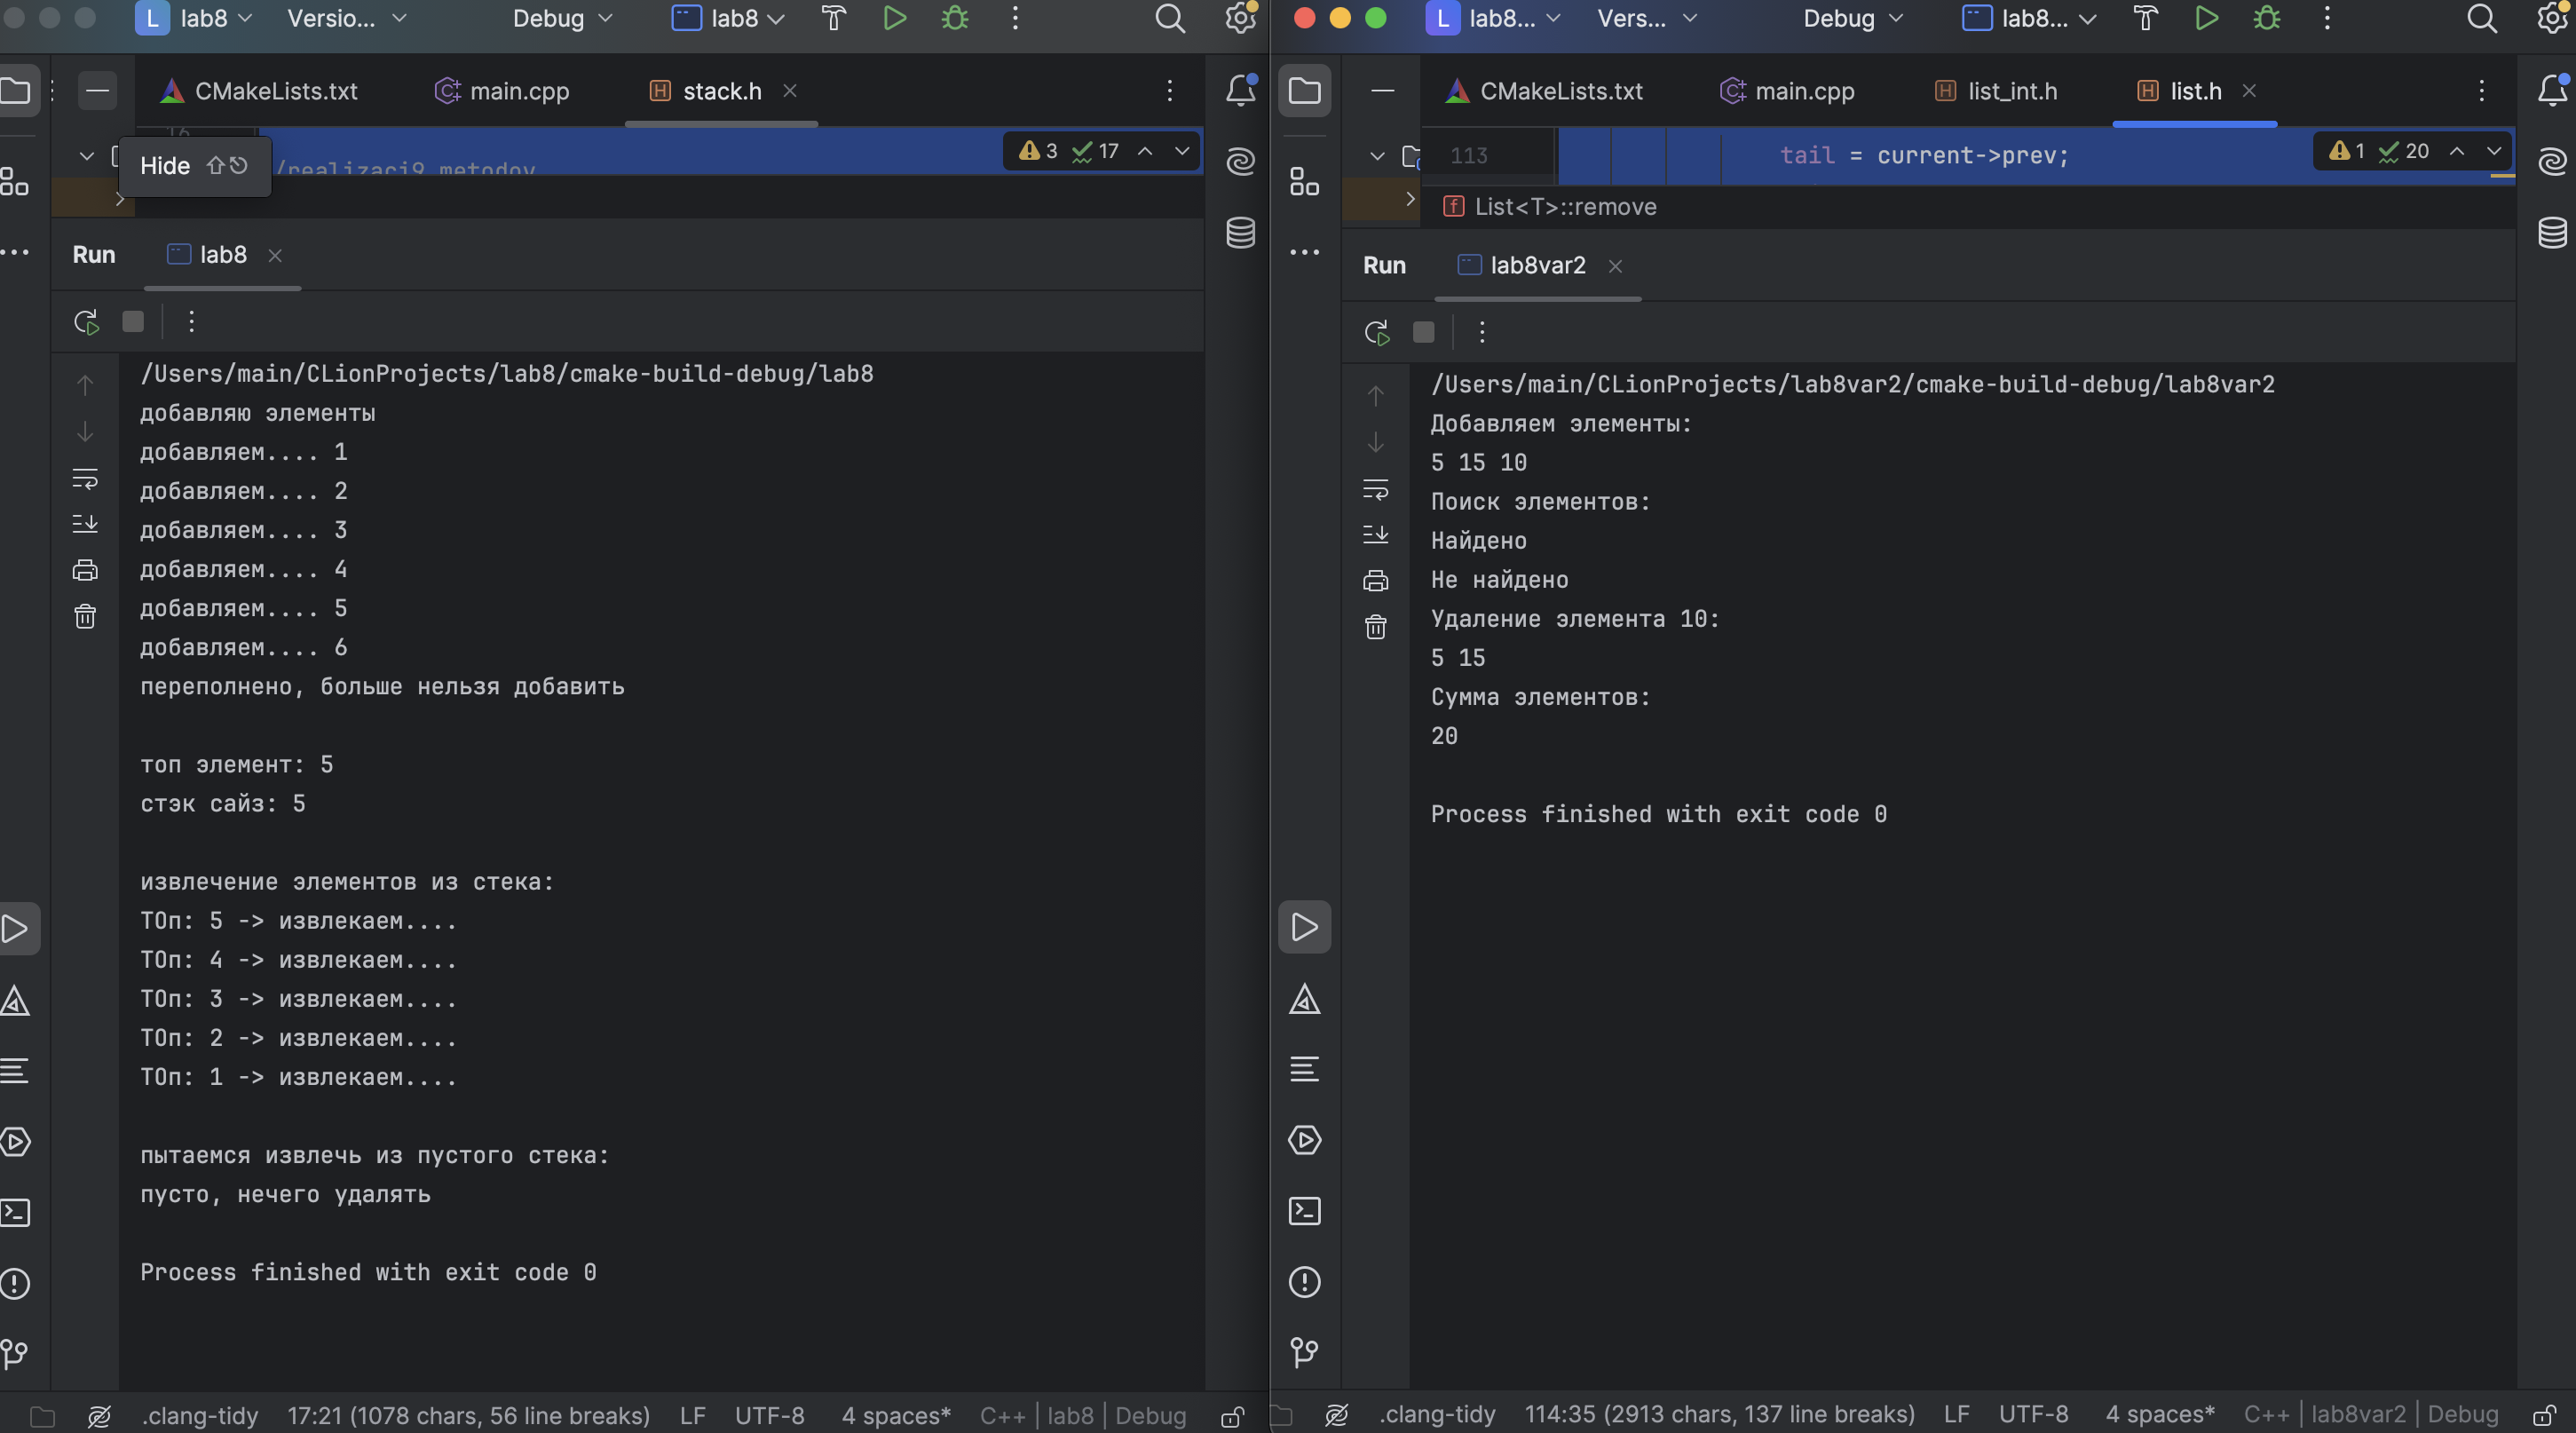
\includegraphics[width=0.8\textwidth]{фото21.jpeg}
  \captionof{figure}{Пример консольного вывода тестовых программ}
\end{center}

%--------------------------------------
\section{Вывод}
В ходе выполнения лабораторной работы были разработаны шаблоны контейнерных
классов и полностью протестированы их основные операции:

\begin{itemize}[nosep]
  \item \textbf{List<T>}~— двусвязный список с операциями вставки в произвольную
        позицию, поиска, удаления, вывода и (для специализации
        \lstinline|int|)~подсчёта суммы элементов.
  \item \textbf{Stack<T,N>}~— параметризуемый стек с ограничением на размер
        (при $N \ne 0$), снабжённый типичными операциями и защитой от выхода
        за пределы ёмкости.
  \item Все классы соблюдают \emph{правило трёх}: реализованы деструкторы,
        конструкторы копирования и операторы присваивания (в рамках
        шаблонов — неявные).
  \item Тестовые программы убедительно демонстрируют корректность работы
        контейнеров и обработку граничных ситуаций (переполнение стека,
        удаление из пустой структуры).
\end{itemize}

Полученные на практике навыки проектирования шаблонных классов и управления
памятью без стандартных контейнеров станут полезной базой для реализации
индивидуальных вариантов \textbf{Equality<T,N>} и \textbf{IntPQueue<L,H>} с
расширенным функционалом.
\end{document}
